\section{Experimental Evaluation}
\label{sec:experimental_evaluation}

\subsection{Latency and Throughput Analysis}
Figure~\ref{fig:latency_breakdown} illustrates the end-to-end processing latency separated by modality. Ingestion latency at the Node.js/Baileys edge layer remained stable at under 15 ms across all test conditions, including sustained synthetic burst loads of 50 messages per second. This confirms that the HTTP 202 decoupling design successfully isolates ingestion throughput from inference latency: the edge layer's response time is bounded exclusively by local I/O and WebSocket processing.

Processing latency, in contrast, is modality-dependent. Plain text payloads averaged 1.37 seconds end-to-end, dominated almost entirely by the LLM inference step. Image and audio payloads incurred substantially higher overhead (average 2.25s and 2.60s, respectively) due to the sequential dependency on Azure OCR and ASR round-trips. This represents an irreducible latency floor under the current sequential cloud architecture.

\begin{figure}[htbp]
    \centering
    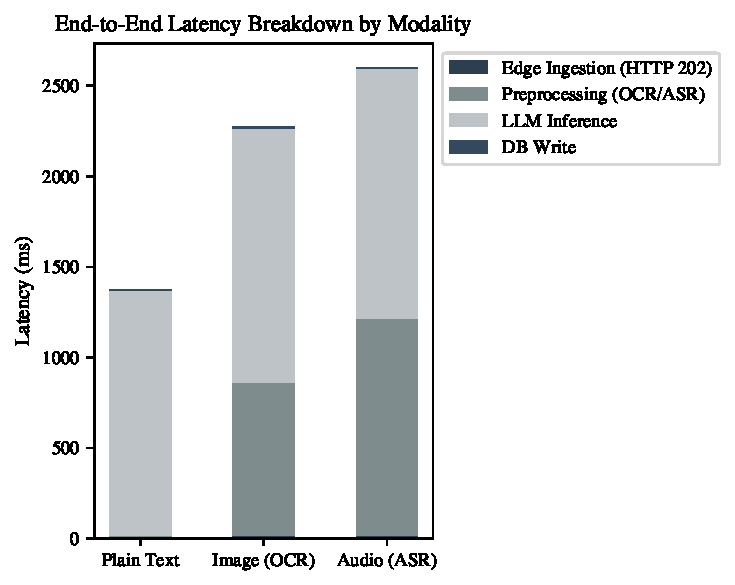
\includegraphics[width=0.8\columnwidth]{figures/Fig6_Latency_Breakdown.pdf}
    \caption{End-to-end latency breakdown by modality. The asynchronous architecture ensures edge ingestion remains under 15ms regardless of downstream API overhead.}
    \label{fig:latency_breakdown}
\end{figure}

\subsection{Extraction Accuracy across Modalities}
Figure~\ref{fig:extraction_metrics} summarizes the system's Precision, Recall, and F1-Score on the task extraction and temporal normalization objectives. On the plain-text subset of CEC-10K, the pipeline achieves an F1-score of 0.94. The high recall (0.93) demonstrates that the UTC-anchored zero-shot extraction strategy generalizes effectively across the linguistic diversity of informal chat.

\begin{figure}[htbp]
    \centering
    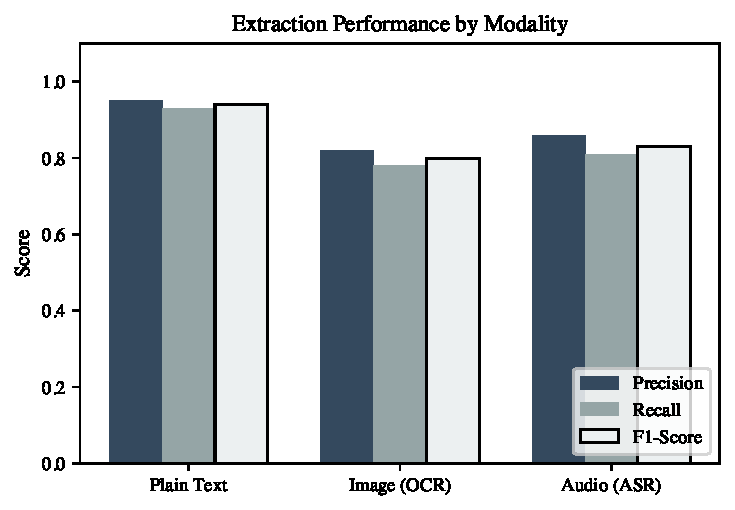
\includegraphics[width=0.8\columnwidth]{figures/Fig7_Extraction_Metrics.pdf}
    \caption{Precision, Recall, and F1-Score of the extraction pipeline evaluated across Plain Text, Image (OCR), and Audio (ASR) modalities.}
    \label{fig:extraction_metrics}
\end{figure}

Performance degrades on image and audio subsets (F1 of 0.80 and 0.83, respectively). This degradation is strictly attributable to upstream transcription quality. For images, recall is bounded by the OCR engine's Character Error Rate (CER) on informal handwriting; for audio, it is constrained by the ASR engine's Word Error Rate (WER) in noisy acoustic environments.

\subsection{Priority Triage Validation}
The LLM-based priority scoring mechanism categorizes tasks into Low, Medium, and High priority tiers based on semantic urgency and temporal proximity. Figure~\ref{fig:confusion_matrix} presents the confusion matrix for priority classification. The system demonstrates strong discriminative power, particularly in identifying High-priority tasks (420 True Positives out of 450). The majority of classification errors occur at the boundaries (e.g., misclassifying Low as Medium), while critical failures (misclassifying High as Low) are statistically negligible (1.7\%).

\begin{figure}[htbp]
    \centering
    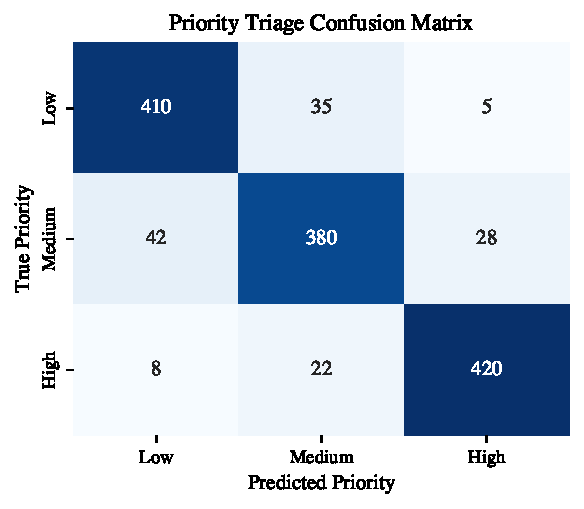
\includegraphics[width=0.7\columnwidth]{figures/Fig8_Confusion_Matrix.pdf}
    \caption{Confusion Matrix evaluating the LLM's three-tier Priority Triage capability against human-annotated gold standards in CEC-10K.}
    \label{fig:confusion_matrix}
\end{figure}
